% =====================================================================================
% HEADLINE CLAIM REFUTED ON REVIEW, 2026-08-02 — THIS DRAFT MUST NOT BE SUBMITTED OR SHARED.
%
% The independent review of the section 11.3 packet returned REVISE and refuted the central
% sentence. "A perfect ranking would clear the 20% floor" is FALSE. The 23.6% oracle acceptance
% is EMPIRICAL and carries no finite-sample penalty; under the certifier's own hoeffding_upper a
% perfect ranking of this population certifies 0.1139 (per-system delta/3) or 0.0838
% (family-wide) — both BELOW the 0.20 floor. At the floor (279 groups) empirical risk is 0.174
% against an upper bound of 0.267-0.283.
%
% This is the same error the paper avoids for the alpha* = 0.406 frontier point, one section
% later, and it runs in the flattering direction.
%
% SURVIVES: the 2.0% vs 23.6% comparison (both empirical, so the 21.6-point gap is still the
%   ranking's). DOES NOT: any claim the target was reachable or the floor would have been cleared.
% AFFECTED: abstract, section 4, section 7 (Conclusion), Figure 1 caption.
%
% Awaiting the owner's decision. Do not edit these passages without it.
% =====================================================================================

% UncertaiNLP 2026 short paper (4 pages). DRAFT — NOT SUBMITTED.
%
% Blocked on two outstanding review packets; see the Markdown source
% (uncertainlp-2026-short.md), which is the authored copy this file is typeset from and which
% carries the full status banner, provenance notes and the remaining-work list.
%
% BUILD (acl.sty is NOT vendored — no upstream licence; see acl-template.md):
%   TEXINPUTS=".;./acl-template;" BIBINPUTS=".;./acl-template;" \
%   pdflatex uncertainlp-2026-short && bibtex uncertainlp-2026-short && pdflatex ... (x2)
% or run scripts/build_paper.ps1 from the repository root.

\documentclass[11pt]{article}
\usepackage[review]{acl}

\usepackage{times}
\usepackage{latexsym}
\usepackage[T1]{fontenc}
\usepackage[utf8]{inputenc}
\usepackage{microtype}
\usepackage{inconsolata}
\usepackage{graphicx}
\usepackage{booktabs}

\title{A well-ranked score that certifies nothing:\\
selective risk control for document-level event-argument extraction}

\author{Anonymous submission}

\begin{document}
\maketitle

\begin{abstract}
Selective prediction is usually judged by how well a confidence score \emph{ranks} correct outputs
above incorrect ones --- AUROC, AURC, rank correlation. Distribution-free risk control asks a
different question: how much output can be accepted while provably bounding error on what is
accepted. We show these can diverge by an order of magnitude on the same system. We define a
frozen, sealed-split selective-certification protocol for document-level event-argument extraction
on RAMS, with the source document as the independent unit and mean bounded frame loss as the
document loss, and run it once on a QLoRA-adapted Qwen3-4B and two prompted baselines. All three
are infeasible at a 20\% risk target with 95\% confidence and a 20\% acceptance floor. The adapted
system's confidence score is \emph{not} weak by selective-prediction standards --- group AUROC
0.796, Spearman $\rho = -0.403$ --- yet it delivers 2.0\% acceptance where a perfect ranking of the
same population reaches 23.6\% and would clear the floor. Risk control needs the top of the ranking
to be nearly clean, not the whole ranking to be ordered, and ranking metrics do not report that. We
also find that the choice of independent unit is itself decisive: mean loss is flat in
triggers-per-document while the share of acceptable documents falls from 17.3\% to zero.
\end{abstract}

\section{Introduction}

Two literatures measure confidence and rarely meet. Selective prediction and hallucination
detection report \textbf{ranking quality}: AUROC for separating correct from incorrect outputs,
area under the risk-coverage curve, rank correlation against loss. Distribution-free risk control
\cite{angelopoulos2024crc} reports \textbf{certified acceptance}: the fraction of inputs a policy
may accept while a finite-sample bound holds on the error rate among accepted inputs.

These are not the same quantity, and the gap between them is not a technicality. A score can order
a population well on average and still fail to isolate a clean prefix --- and it is the prefix, not
the ordering, that a certificate needs. This paper reports a case where that gap is an order of
magnitude, on a task where both numbers are worth having.

\paragraph{What we contribute.} We state up front what is \emph{not} new. That conformal risk
control frequently cannot certify LLM outputs, that base risk $\mu$ forces abstention of at least
$(\mu-\alpha)/(1-\alpha)$, and that this bites across multiple systems, are all established by
\citet{kotte2026crc}, which we read on 2026-07-18 and folded into this study's design three days
before its parameters were frozen. Roughly 80\% of what we measured is a replication of that work
in a new task. Three things are ours:

\begin{enumerate}
\item \textbf{A protocol} (\S\ref{sec:protocol}): a frozen, sealed-split certification for
  event-argument extraction at the \textbf{source-document} unit, with mean bounded frame loss as
  the document loss. \citet{kotte2026crc} evaluates no event-argument extraction; we found no prior
  application of distribution-free risk control at this unit for this task, though we have not run
  a systematic survey.
\item \textbf{The ranking/certification divergence} (\S\ref{sec:divergence}): the paper's main
  finding, and the one an uncertainty audience can act on.
\item \textbf{A dissociation between grounding and certifiability} (\S\ref{sec:grounding}),
  measured rather than asserted.
\end{enumerate}

\section{Protocol}
\label{sec:protocol}

\paragraph{Task and unit.} RAMS \cite{ebner2020rams}, in-domain. A system may \textbf{abstain} on a
document rather than emit event frames. The independent unit is the \textbf{source document}, which
we call a \emph{group} because one source document carries one or more trigger instances: it is the
level at which the corpus has near-duplicates, so it is the level at which independence is
defensible. \textbf{Group loss} is the mean bounded frame loss over the document's triggers
($1 - $ span-exact micro-F1 per frame); a structurally invalid or ungrounded output scores 1.0 and
is never rewarded for content it did not produce. \textbf{Group score} is the \textbf{minimum}
confidence over the group's instances, and a group is eligible for acceptance only if
\textbf{every} instance parsed and grounded. Accepting the weakest member's score and averaging the
loss is a deliberate pairing --- it is what makes acceptance a statement about the whole document
--- and \S\ref{sec:divergence} shows it is also consequential.

\paragraph{Target, frozen before any sealed label was read.} Risk $\alpha = 0.20$, confidence
$\delta = 0.05$, acceptance floor 0.20. The target is a commitment this study made, not a natural
constant. Nothing below relaxes it and no certificate is issued at any other operating point.

\paragraph{Systems.} Zero-shot (ZS), few-shot (FS), and a QLoRA-adapted (QA)
Qwen3-4B-Instruct-2507, all served on one frozen 4-bit vLLM stack. Confidence is mean transition
log-probability over the parsed object; two alternatives (10th percentile, minimum) were
pre-registered and are reported.

\paragraph{Discipline.} The certification split was opened \textbf{exactly once} --- 3,152
documents forming 1,396 groups --- under a hash-chained access log, with zero reads of the held-out
\texttt{final} and \texttt{shift} splits, which remain sealed. Certification and all analysis ran
on CPU at no cost; the GPU programme totalled about \$18.7--18.9.

\section{The null}

\textbf{No system certifies.} All three are infeasible under the primary construction and under a
conservative audit. Because both baselines are infeasible, the two pre-registered comparisons
collapse to \textbf{one} finding, not two, and no numerical difference is computed against an
infeasible baseline.

The result is not an artefact of the bound. Under an \textbf{oracle} reading --- unlimited
threshold grid, zero finite-sample penalty, threshold chosen with the labels in hand --- the best
system still accepts at most \textbf{2.0\%} of documents at 20\% empirical error, against a floor
of 20\%. The same diagnostic on the development split gives 3.0\%, so it reproduces out of sample.
Nor is the target a specially unlucky choice: on the oracle risk-coverage curve the 20\% floor
first becomes reachable at \textbf{empirical oracle frontier points} of 0.406 (QA), 0.930 (FS) and
0.981 (ZS). These are frontier points measured after the split was opened, from its own labels ---
\textbf{not thresholds, and not certified operating points}. The curve rules operating points out;
it never rules one in, and no claim here uses it in that direction.

\begin{table}[t]
\centering
\small
\setlength{\tabcolsep}{4pt}
\begin{tabular}{@{}lrrr@{}}
\toprule
Certification split & ZS & FS & \textbf{QA} \\
\midrule
base risk $\mu$ (group)          & 0.9923 & 0.9580 & \textbf{0.6071} \\
ineligible groups                & 1,020  & 684    & \textbf{130} \\
bound $1-(\mu-\alpha)/(1-\alpha)$ & 0.0096 & 0.0525 & \textbf{0.4911} \\
\textbf{loss-optimal oracle}     & 0.0036 & 0.0244 & \textbf{0.2357} \\
acceptance delivered             & 0.0000 & 0.0000 & \textbf{0.0201} \\
AUROC (error detection)          & 0.344  & 0.727  & \textbf{0.796} \\
normalized AURC                  & 0.926  & 0.920  & \textbf{0.531} \\
Spearman $\rho$ vs.\ loss        & $-$0.027 & $+$0.073 & \textbf{$-$0.403} \\
\bottomrule
\end{tabular}
\caption{All 1,396 certification groups, each system at the confidence candidate its development
gate selected (QA and ZS mean, FS 10th percentile). ``Ineligible'' groups contain a structurally
invalid or ungrounded member and can never be accepted. Normalized AURC is 0 for a perfect ranking
and 1 for chance. All nine system~$\times$~candidate combinations are in the released artifact.}
\label{tab:main}
\end{table}

\paragraph{Two different failures, which must not be merged.} For ZS and FS the arithmetic settles
it: base risks of 0.992 and 0.958 permit at most 0.96\% and 5.25\% acceptance, and their
loss-optimal oracles are 0.36\% and 2.44\% --- an order of magnitude below the floor.
\textbf{No score whatever could certify them.} QA is the interesting case.

\section{Ranking quality does not transfer to certified acceptance}
\label{sec:divergence}

Read as a selective-prediction result, QA's confidence score is respectable. Group AUROC for error
detection is \textbf{0.796}. Rank correlation against group loss is $\rho = -0.403$ at
$p \approx 10^{-55}$, and a normalized AURC of \textbf{0.531} says the score closes roughly half
the distance between a random ranking and a perfect one. On the development split the same figures
are 0.834, $-0.313$ and 0.568.

Table 5 of \citet{kotte2026crc} gives the natural comparison, and it is a close one.
Log-probability scores there reach AUROC 0.485--0.604 across NER, QA and classification --- but
\textbf{0.793 on JSON extraction}, the one structured-generation task in that paper. Our 0.796 sits
almost exactly on it. Two independent studies therefore find log-probability confidence
discriminating errors at close to 0.80 AUROC on structured generation, and the comparison is worth
making precisely because the certification outcomes diverge completely: JSON extraction has base
risk 0.033 and certifies easily, ours has 0.6071 and does not. \textbf{The score quality is the
same; the certified acceptance is not.} (Not a like-for-like measurement --- theirs is
instance-level and ours is group-level over documents --- so the agreement is indicative rather
than exact.)

Read as a risk-control result, the same score is close to useless. It delivers \textbf{2.0\%}
acceptance at $\alpha = 0.20$. A perfect ranking of the identical population delivers
\textbf{23.6\%} --- which clears the 20\% floor. \textbf{The target was reachable by ranking alone,
and the score reached less than a tenth of what was available.} Figure~\ref{fig:rc} is that
sentence as a picture.

\begin{figure*}[t]
\centering
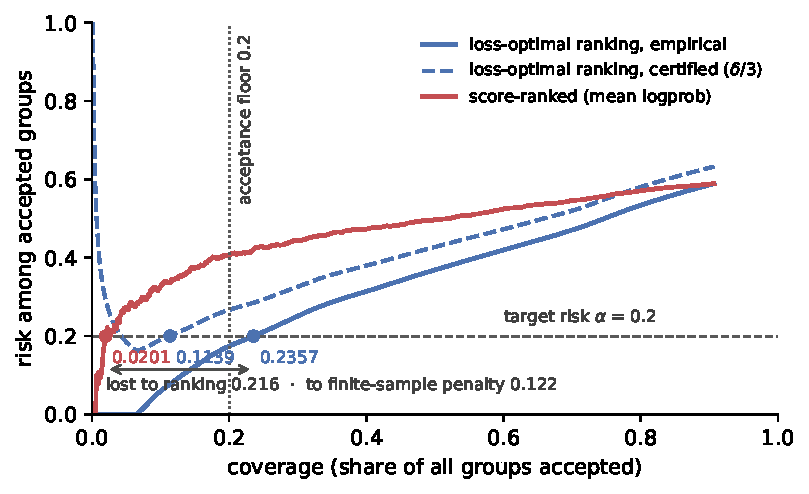
\includegraphics[width=0.72\textwidth]{fig/risk-coverage-qa.pdf}
\caption{Risk-coverage curves for the QLoRA system on the certification split. Both curves cover
the same 1,396 groups and differ only in how they are ranked: red accepts best-scoring groups first
(what the certifier sweeps), blue accepts lowest-loss groups first (what a perfect ranking would
reach). Where each crosses the $\alpha = 0.20$ rule is the acceptance it supports --- 0.0201
against 0.2357. The acceptance floor at 0.20 sits between them, so the blue curve clears the target
and the red does not. The gap between the crossings, 0.216, is attributable to the ranking alone:
the population is held fixed.}
\label{fig:rc}
\end{figure*}

We report that gap against the loss-optimal oracle rather than against the arithmetic bound, and
the distinction matters. The bound $1-(\mu-\alpha)/(1-\alpha)$ gives 49.1\% for this population,
but it assumes the population's ``goodness'' can be concentrated arbitrarily, which this population
does not supply. Quoting 49.1\% would charge the score for 25 points that were never on offer. The
honest shortfall is \textbf{21.6 points, not 47}.

\paragraph{Why good ranking does not buy a certificate.} A certificate at $\alpha$ needs the
accepted \emph{prefix} to average below $\alpha$. Global ordering quality does not guarantee that
any prefix is clean enough. QA's best-scoring 5\% of groups still average \textbf{0.274} loss; at
10\% coverage, 0.324; at 20\%, 0.405. The running risk never drops below the target at any coverage
worth having. AUROC integrates over all pairs and is dominated by the bulk of the distribution,
where this score does order documents sensibly; the certificate depends entirely on the extreme
tail, where it does not.

This is the practical message for uncertainty work: \textbf{an AUROC in the 0.8 range is not
evidence that a score can support risk-controlled selective prediction.} The two should be reported
together, and where a paper reports only ranking metrics, the certified quantity may be an order of
magnitude worse.

\paragraph{The unit definition is also decisive}, and this is easy to miss. Stratifying QA's groups
by number of triggers per document, mean group loss is essentially flat (0.606, 0.608, 0.589,
0.634, 0.596 from 1 to 6+ triggers) --- but the share of groups whose loss is within $\alpha$
collapses from \textbf{17.3\% to 0.7\% to zero}, and 23 of the 28 oracle-accepted groups are
single-trigger documents. Groups with three or more triggers contribute \textbf{none}. Averaging
frame loss across a document and scoring the group by its weakest member makes acceptance vanish
with document complexity even where mean loss does not move. Cross-sentence argument distance
behaves the same way: 25 of 28 acceptances have no cross-sentence argument, and groups with three
or more contribute none. A protocol that reports only aggregate loss will not see either effect.

\section{What the adapter changed, and what it did not}
\label{sec:grounding}

QLoRA adaptation produced a large, real improvement in \textbf{grounding fidelity}: 95.7\% of QA
outputs parse and ground to the source document against 39.4\% zero-shot and 68.1\% few-shot, with
ungrounded spans falling from 5,355 to 340. ``Valid'' here means parseable and grounded,
\textbf{not correct} --- a span can point at real document text and still name the wrong entity or
role --- and \textbf{this improvement did not translate into a certified selective guarantee}.
Neither half of that sentence may be reported without the other.

Decomposing loss into four channels says why. The ${\sim}16\times$ separation in ungrounded spans
lives in the channels that are forced to loss 1.0 or are contentless. The certificate scores the
fourth channel --- well-formed, grounded, content-bearing output --- which holds \textbf{90.3\%} of
QA's documents and \textbf{87\%} of its loss, at a within-channel mean loss of 0.579. The adapter
moved the channels the certificate does not score and left the one it does.

\textbf{This is a dissociation, not an orthogonality result.} One intervention observed across three
systems cannot establish that two properties are independent, and we did not test independence. At
group level the two are in fact weakly associated --- grounded share against group loss gives
$\rho = -0.206$ at $p \approx 8\times10^{-15}$ --- but the 1,266 QA groups whose every member is
grounded still average \textbf{0.589} loss, roughly three times the target. Grounding was necessary
and nowhere near sufficient.

The decomposition locates loss by channel; it does \textbf{not} identify the error category that
produced it, and we claim none. An earlier version of this claim attributed the residual to output
``that names the wrong entity''; that rested on unquantified inspection of two development examples
and was withdrawn on independent review. A measurement points elsewhere --- on these frames false
positives exceed false negatives by 637 arguments, which is over-generation rather than
entity-naming.

\section{Relation to prior work}

\citet{kotte2026crc} establishes the impossibility bound, the base-risk feasibility test, and
infeasibility across multiple systems; we reproduce all three in a new task and at a new unit. Our
measured base risk (0.6071) is \textbf{not} a reproduction of their extraction figure and does not
contradict it: their one extraction task, JSON-Extract, sits at $\mu = 0.033$, a different task
under a different metric. The comparison marks out a harder operating regime and settles nothing
about their number.

\textbf{This is not a task-wide impossibility, and must not be read as one.} A 20\% target is
demonstrably reachable on structured extraction: $(\mu-\alpha)/(1-\alpha)$ forbids nothing at
$\mu = 0.033$ and permits up to 80.5\% acceptance at $\mu = 0.356$, the easiest NER dataset
\citet{kotte2026crc} reports. What we establish is that \emph{this} model with \emph{this} score on
\emph{this} task at $\mu = 0.6071$ could not --- a model- and score-specific result.

The score-quality comparison in \S\ref{sec:divergence} is with that paper's Table 5 rather than
with the semantic-entropy literature, for a reason worth stating: within that one table,
log-probability reaches 0.793 on structured extraction while semantic entropy reaches only
0.496--0.677 across all eight datasets. Which uncertainty score is strongest is evidently
setup-dependent, and our finding does not need that question settled --- it needs only that the
score we used is a normal one, performing about as well as its family does elsewhere on this kind
of task. It is.

\section{Conclusion}

On document-level event-argument extraction, a confidence score with AUROC 0.796 and
$\rho = -0.403$ delivered 2.0\% certified-eligible acceptance where a perfect ranking of the same
population reached 23.6\% and would have cleared the 20\% floor. Ranking quality and certified
acceptance are different measurements and can differ by an order of magnitude.
Selective-prediction work that reports only the former should not be read as evidence about the
latter.

\section*{Limitations}

\textbf{Not production-grade}, and no deployment claim is made. \textbf{The certificate bounds
average within-group loss, not the absence of error} in any document; certified $\neq$ safe.

\textbf{The system is not competitive on extraction quality.} Group loss 0.6071 corresponds to a
mean per-document span-exact F1 of about 0.393. That is a mean of per-document F1 at the
source-document unit and is \textbf{not} directly comparable to corpus-level micro Arg-C figures
such as the 54.4 of \citet{huang2026rose}, but the gap is real and large; we make no claim about
competitiveness.

\textbf{Single seed, no training ablations.} One frozen 4-bit vLLM serving stack, with 86.3\%
parsed-output agreement measured against the training stack; the abstain/extract decision itself
flips between stacks at 1.3--1.8\% of frames at plausible operating points. Portability is not
established.

\textbf{In-domain RAMS only}, under span-exact matching. The held-out \texttt{final} and
\texttt{shift} splits are descoped and remain sealed; no distribution-shift claim is made in either
direction.

\textbf{The empirical oracle frontier points and the \S\ref{sec:divergence} diagnostics are
post-hoc on an opened split.} They select no threshold and certify nothing.

\textbf{The infeasibility was knowable for \$0 before the sealed split was opened}: the
development-split oracle diagnostic already showed 3.0\% against a 20\% floor and neither the
implementer nor the reviewer ran it. Recorded as a joint process failure.

\textbf{The self-consistency alternative was not tested.} Agreement-based scores reach AUROC
0.600--0.816 across the eight datasets of \citet{kotte2026crc} and might behave differently here;
we did not run it. Our finding is about one score family --- transition log-probability --- and does
not show that no score can certify this task.

\section*{Reproducibility}

The protocol, certifier, diagnostics and claim ledger are code, and every figure above resolves to a
committed artifact. Released with publication: source, the frozen group mapping, per-system
predictions with confidence candidates, and the certification and diagnostic artifacts. Raw corpus
text and sealed labels are not redistributable.

\bibliography{uncertainlp-2026-short}

\end{document}
